%!TEX root = ./template-skripsi.tex
%-------------------------------------------------------------------------------
%                     BAB III
%               			PEMBAHASAN
%-------------------------------------------------------------------------------
% \SetKwComment{Comment}{/* }{ */}
\chapter{METODOLOGI PENELITIAN}

\section{Perancangan Sistem}

Penulis merancang sistem ini berdasarkan dari 
penelitian Rizki, yaitu untuk pendeteksian luka. 
Yang membuat penelitian ini berbeda dengan penelitian 
Rizki adalah interpolasi yang dipakai adalah buatan 
penulis dengan referensi NURBS, lalu menggantikan 
\textit{active contour} dengan \textit{border following} 
yang ditulis oleh Hafizhun Alim(\cite{Hafizhun}). berikut merupakan diagram 
alir penelitian yang akan dilakukan.

\begin{figure}[H]
	\centering
	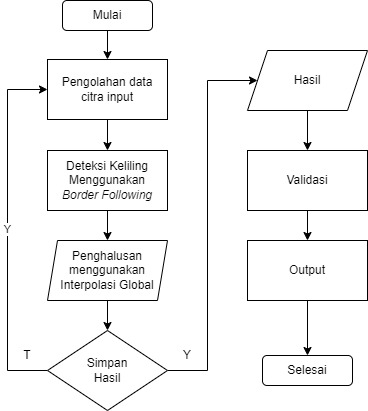
\includegraphics[keepaspectratio,width = 7cm]{gambar/Bab3Extra/Diagram_alur.jpg}
	\caption{Diagram alir penelitian}
	\label{diagramalur}
\end{figure}

\begin{algorithm}[H]
  \caption{\textit{Main}}
  \begin{algorithmic}[1]
  \Require{Image, $p$}
  \Ensure{Curve Points}
  \Function{Main}{Image, $p$}
    \State image $\gets$ imread(Image) \Comment read image as value
    \State points $\gets$ BorderFollowing(image) \Comment algorithm(\ref{algoritma:BorderFollowing})
    \State curve $\gets$ GlobalInterpolation(points, $p$) \Comment algorithm(\ref{algoritma:globalinterpolation})
    \State Results $\gets$ Image + curve \Comment put curve to image
    \State \Return Results
  \EndFunction
  \end{algorithmic}
  \label{algoritma:main}
\end{algorithm}

\section{\textit{Border Following}}

Setelah citra diolah 

Setelah merubah gambarnya dengan Interpolasi, penulis 
akan menggunakan teknik \textit{border following} untuk membuat garis 
pada gambar. \textit{Border following} merupakan teknik yang diusulkan 
oleh Satoshi Suzuki dan Keichi Abe di mana teknik ini menelusuri 
batas suatu objek dengan mengikuti transisi antara piksel latar 
depan (objek) dan latar belakang pada gambar lalu memberikan 
definisi derajat pada piksel. Algoritma \textit{border following} bekerja 
dengan memulai pada titik tertentu pada batas suatu objek dan 
kemudian mengikuti batas tersebut searah atau berlawanan 
arah jarum jam dengan mengidentifikasi titik berikutnya di 
sepanjang batas tersebut.

Algoritma ini dimulai dengan mengasumsikan citra yang 
dimasukkan merupakan citra biner dengan latar belakang 
merupakan piksel bernilai 0 dan latar depan (objek) 
sebagai piksel bernilai 1. Lalu dilanjutkan dengan 
memberi masukan berupa citra biner dari proses operasi 
morfologi yang dilanjutkan denang proses memindai(scan) 
dimulai dari piksel paling kiri atas. Apabila sudah memindai
sampai piksel ($i, j$) bernilai $f_{i,j} \neq 0$ (bukan latar
belakang), ditentukan piksel tersebut apakah merupakan 
\textit{starting point}  dari operasi \textit{border following}
untuk tepi luar atau tepi dalam (gambar \ref{gambar:kondisi_batas}).
Lalu menentukan \textit{parent border} untuk piksel 
(i,j) berdasarkan gambar (\ref{gambar:hasil_penciutan_blob}).
Dilanjutkan dengan melakukan \textit{border following} dimulai 
dari \textit{starting point} piksel (i, j) sampai 
\textit{pointer} kembali ke posisi \textit{starting point}.
Algoritma yang dipakai adalah algoritma kedua Suzuki(\cite{Suzuki})
maka nilai $N B D$ dan $- N B D$ akan di-set 
masing-masing 2 dan -2. lalu pemindai akan melanjutkan pemindaian
untuk mencari objek ($f_{i,j} \neq 0$). Algoritma ini selesai
apabila pemindai sudah sampai sudut kanan bawah.
\begin{algorithm}[H]
  \caption{\textit{Main Border Following}}
  \begin{algorithmic}[1]
  \Require{image, start, previous}
  \Ensure{contour}
  \Function{BorderFollowing}{self, image, start, previous}
    \State pointer$\_$one $\gets$ previous
    \State pointer$\_$three $\gets$ start
    \State contour[]
    \Statex
    \State \# clockwise movement
    \State count $\gets$ 0
    \While{image[pointer$\_$one[0]][pointer$\_$one[1]] = 0}
      \If{count > 7} \Comment{If the starting pixel is a single pixel dot}
        \State image[pointer$\_$one[0]][pointer$\_$one[1]] = 4
        \State contour $\gets$ image[pointer$\_$one[1]-1][pointer$\_$one[1]-1]
        \State \Return contour
      \EndIf
      \State position, next pointer $\gets$ next pointer position clockwise
      \State pointer$\_$one $\gets$ next pointer
      \State count $\gets$ count + 1
    \EndWhile
    \State pointer$\_$two $\gets$ copy of pointer$\_$one
    \State counter $\gets$ 0
    % potong
    \algstore{bordfol}
  \end{algorithmic}
  \label{algoritma:BorderFollowing}
\end{algorithm}

\begin{algorithm}[H]
  \begin{algorithmic}[1]
    \algrestore{bordfol}
      \While{True}
      \State \# Counter clockwise movement
      \State position, next pointer $\gets$ next pointer position counter clockwise
      \State pointer$\_$two $\gets$ next pointer
      \While{image[pointer$\_$two[0]][pointer$\_$two[1]] = 0}
        \State position, next pointer $\gets$ next pointer position counter clockwise
        \State pointer$\_$two $\gets$ next pointer
      \EndWhile
      \State pointer$\_$four $\gets$ pointer$\_$two
      \State \# Assign NBD
      \State NBD$\_$coordinate $\gets$ copy pointer$\_$three
      \If{image[NBD$\_$coordinate[0]][NBD$\_$coordinate[1]+1] = 0}
        \State image[NBD$\_$coordinate[0]][NBD$\_$coordinate[1]] = 4
      \ElsIf{image[NBD$\_$coordinate[0]][NBD$\_$coordinate[1]+1] $\neq$ 0 and image[NBD$\_$coordinate[0]][NBD$\_$coordinate[1]] = 1}
        \State image[NBD$\_$coordinate[0]][NBD$\_$coordinate[1]] = 2
      \EndIf
      \State contour $\gets$ image[NBD$\_$coordinate[1]-1][NBD$\_$coordinate[0]-1]
      \Statex
      \State \# Determine new pointer or break
      \If{pointer$\_$four[0] = start[0] and pointer$\_$four[1] = start[1]}
        \If{pointer$\_$three[0] = pointer$\_$one[0] and pointer$\_$three[1] = pointer$\_$one[1]}
          \State break
        \EndIf
      \EndIf
      \State pointer$\_$two $\gets$ copy of pointer$\_$three
      \State pointer$\_$three $\gets$ copy of pointer$\_$four
      \State counter $\gets$ counter + 1
    \EndWhile
    \State \Return contour
  \EndFunction
  \end{algorithmic}
\end{algorithm}

\section{Interpolasi}

Setelah mendapatkan titik koordinat dari hasil pemindaian 
dari border following, maka akan dilanjutkan dengan 
penghalusan kurva oleh interpolasi. Interpolasi yang 
digunakan oleh penulis merupakan 
\textit{surface fitting interpolation} di mana teknik 
ini digunakan untuk membuat permukaan halus yang melewati 
titik dari poin data yang diberikan. Dalam konteks gambar, 
\textit{surface fitting interpolation} juga bisa digunakan untuk 
membuat permukaan halus dan kontinu yang merepresentasikan 
nilai intensitas gambar pada setiap lokasi piksel.

Berdasarkan hasil penelitian Rizki, interpolasi ini 
meningkatkan akurasi dari alat deteksinya, dari yang 
normalnya mendapatkan 77.18\% menjadi 86.1\%. Penulis 
menginginkan untuk mengembangkan angka itu dengan meneliti 
cara kerja algoritma interpolasi rizki, menjadi buatan sendiri 
yang bisa diatur algoritmanya.

\begin{figure}[H]
	\centering
	\begin{subfigure}{.3\textwidth}
		\centering
		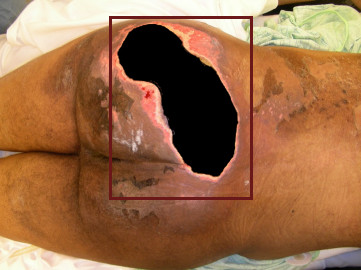
\includegraphics[keepaspectratio, width=3cm]{SourceCode/dataset/luka_hitam/41.jpg}
		\caption{Luka Hitam di-\textit{crop}}
	\end{subfigure}
	\begin{subfigure}{.3\textwidth}
		\centering
		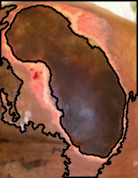
\includegraphics[keepaspectratio, width=3cm]{gambar/Bab3Extra/LukaHitamBorderFollowing.jpg}
		\caption{pindai luka hitam}
	\end{subfigure} 
	\begin{subfigure}{.3\textwidth}
		\centering
		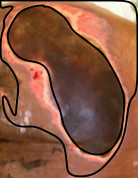
\includegraphics[keepaspectratio, width=3cm]{gambar/Bab3Extra/LukaHitamCurve.jpg}
		\caption{Luka diinterpolasi}
	\end{subfigure}
	\caption{Hasil Interpolasi citra}
\end{figure}

Seperti di penelitian Rizki, untuk mendapatkan hasil yang lebih 
akurat, dilakukan anotasi terlebih dahulu sehingga mengurangi 
kemungkinan untuk mendapatkan \textit{image noise} atau penggarisan 
tidak perlu pada hasil pendeteksian luka. 

Untuk membuat program interpolasi ini, dibuat dulu variabel
yang diperlukan untuk menjalankan rumus utama. Variabel
yang pertama dicari adalah $\bar{u}$ atau disebut \textit{knot} menggunakan
rumus \textit{chord length} (\ref*{chordlength2}), yang dihitung dengan
memasukkan sejumlah koordinat, lalu dihitung setiap panjang antara koordinat.
Setelah mendapatkan semua panjangnya, lalu ditotalkan untuk menjadi pembagi
sehingga didapatkan $\bar{u}$ sesuai dengan jumlah koordinatnya.
\begin{algorithm}[H]
  \caption{\textit{Chord Length}}
  \begin{algorithmic}[1]
  \Require{\{$\textbf{Q}_k\},k = 0,\dots, n$}
  \Ensure{$\bar{u}$[$n$]}
  \Function{ChordLength}{$\textbf{Q}_k$[$n$]}
    \State {$\bar{u}$[$n$]}
    \State {$\bar{u} \gets$ 0}
    \State {d $\gets$ 0}
    \For{$i \gets 0$ to $n$} \Comment{search of d (total length)}
      \State length $\gets$ $|\textbf{Q}_k - \textbf{Q}_{k-1}|$
      \State $d \gets d +$ length
      \State $\bar{u}$[$i$] $\gets d$
    \EndFor
    \For{$i \gets 0$ to $n$} \Comment{search of knots}
      \State $\bar{u}$[$i$] $\gets$ $\bar{u}$[$i$] $/ d$
    \EndFor
    \State \Return $\bar{u}$[$n$]
  \EndFunction
  \end{algorithmic}
  \label{algoritma:chordlength}
\end{algorithm}
\begin{itemize}
  \setlength{\itemsep}{0pt}
  \setlength{\parskip}{0pt}
  \setlength{\parsep}{0pt}
  \item $\{\textbf{Q}_k\}$ meurpakan input koordinat
  \item $k$ adalah indeks dari koordinat
  \item $n$ jumlah koordinat yang dimasukkan
  \item $\bar{u}$ \textit{knot}, hasil dari algoritma
\end{itemize}

Dari algoritma (\ref{algoritma:chordlength}), didapatkan array 
yang berisikan $\bar{u}$. Variabel selanjutnya adalah $U$ yang 
disebut juga \textit{knot vector} menggunakan rumus rata-rata 
knot (\ref*{penjarakanrata_rataknots}). Dimulai dengan mengambil
hasil dari algoritma {\ref{algoritma:chordlength}} lalu isi array
dengan indeks dari 0 sampai sederajatnya menjadi 0 dan mengisi
array dengan indeks setelah jumlah indeks dikurangi derajat dengan
angka 1. Diantara dari 0 dan 1, diisi dengan menghitung jumlah knot
didalam indeks yang tidak diubah, lalu dibagi dengan derajatnya.
\begin{algorithm}[H]
  \caption{Rata-rata Knot}
  \begin{algorithmic}[1]
  \Require{$\bar{u}$[$n$] and $p$}
  \Ensure{$U$[$n + p + 1$]}
  \Function{KnotVector}{$\bar{u}$[$n$], $p$}
    \State {$U$[$n + p + 1$] }
    \For{$i$ $\gets$ 0 to $n$}
      \If{$i \leq p$}
        \State $U$[$i$] $\gets 0$
      \ElsIf{$i \geq n - p - 1$}
        \State $U$[$i$] $\gets 1$
      \Else
        \State $U$[$i$] $\gets 0$
        \For{$ii \gets i-p$ to $i$}
          \State $U$[$i$] $\gets$ $U$[$i$] + $\bar{u}$[$ii$]
        \EndFor
        \State $U$[$i$] = $U$[$i$] $/ p$
      \EndIf
    \EndFor
    \State \Return $U$[$n + p + 1$]
  \EndFunction
  \end{algorithmic}
  \label{algoritma:knotvektor}
\end{algorithm}
\begin{itemize}
  \setlength{\itemsep}{0pt}
  \setlength{\parskip}{0pt}
  \setlength{\parsep}{0pt}
  \item $\bar{u}$ \textit{knot} yang didapat dari 
  algoritma (\ref{algoritma:chordlength})
  \item $n$ jumlah \textit{knot}
  \item $p$ merupakan derajat interpolasi
  \item $U$ \textit{knot vector}, hasil dari algoritma(\ref{algoritma:knotvektor})
\end{itemize}

Setelah mendapat dua variabel penting yaitu $\bar{u}$
dan $U$, sudah bisa menjalankan rumus dasar (\ref*{rumusdasarN}).
Algoritma dimasukkan empat variabel, yaitu \textit{knot} yang didapatkan
dari algoritma (\ref{algoritma:chordlength}), indeks, derajat, dan
\textit{knot vector} dari algoritma (\ref{algoritma:knotvektor}).
Yang pertama diperiksa adalah apakah derajatnya merupakan nol.
apabila derajatnya nol maka akan diperiksa \textit{knotnya} melebihi 
atau sama dengan \textit{knot vector} pada indeksnya dan kurang 
dari \textit{knot vector} dengan indeks selanjutnya. apabila
iya akan diberika angka satu, apabila tidak akan diberikan nol.
Selain dari derajat nol, maka algoritma ini akan menjadi rekursif
di mana akan selalu memanggil hasil dari derajat sebelumnya.
\begin{algorithm}[H]
  \caption{Rumus Dasar Spline (\textit{B-Spline})}
  \begin{algorithmic}[1]
  \Require{$\bar{u}$, $i$, $p$, $U$[\;]}
  \Ensure{spline}
  \Function{Spline}{$\bar{u}$, $i$, $p$, $U$[\;]}
    \If{$p$ is 0}
      \If{$U$[$i$] $\leq$ $\bar{u}$ < $U$[$i$+1]}
        \State \Return 1
      \Else
        \State \Return 0
      \EndIf
    \Else \Comment{separate left and right equation}
      \State left $\gets$ ($\bar{u}$ - $U$[$i$]) $/$ ($U$[$i+p$] - $U$[$i$])
      \State right $\gets$ ($U$[$i+p+1$] - $\bar{u}$) $/$ ($U$[$i+p+1$] - $U$[$i+1$])
      \State left $\gets$ left * Spline($\bar{u}$, $i$, $p-1$, $U$[\;]) \Comment{recursive}
      \State left $\gets$ right * Spline($\bar{u}$, $i+1$, $p-1$, $U$[\;])
      \State \Return left + right
    \EndIf
  \EndFunction
  \end{algorithmic}
  \label{algoritma:spline}
\end{algorithm}
\begin{itemize}
  \setlength{\itemsep}{0pt}
  \setlength{\parskip}{0pt}
  \setlength{\parsep}{0pt}
  \item $\bar{u}$ \textit{knot} yang didapat dari 
  algoritma (\ref{algoritma:chordlength})
  \item $i$ indeks yang akan dipakai pada algoritma(\ref{algoritma:globalinterpolation})
  \item $p$ merupakan derajat interpolasi
  \item $U$ \textit{knot vector}, didapat dari algoritma(\ref{algoritma:knotvektor})
\end{itemize}

Sebelum langkah terakhir adalah membuat matriks dari rumus (\ref{rumus:Global})
memanggil algoritma (\ref{algoritma:chordlength}), (\ref{algoritma:knotvektor}), 
dan (\ref{algoritma:spline}) yang lalu di \textit{inverse}-nya 
dikalikan dengan koordinat input.
\begin{algorithm}[H]
  \caption{\textit{Global Interpolation}}
  \begin{algorithmic}[1]
  \Require{\{$\textbf{Q}_k\},k = 0,\dots,n$, $p$}
  \Ensure{Curve Points}
  \Function{GlobalInterpolation}{$\textbf{Q}_k$[$n$], $p$}
    \State {$\bar{u}$ $\gets$ ChordLength($\textbf{Q}_k$[$n$])}
    \State {$U$ $\gets$ KnotVector($\bar{u}$, $p$)}
    \State {$\textit{C}$[$n_x$, $n_y$]}
    \For {$y$ $\gets$ 0 to $n_y$}
      \For {$x$ $\gets$ 0 to $n_x$}
        \State $\textit{C}$[$x,y$] = Spline($\bar{u}$[$x$], $y$, $p$, $U$)
      \EndFor
    \EndFor
  \State $\textit{C}$ $\gets$ Inverse$\_$of$\_$$\textit{C}$ * $\textbf{Q}$
  \State \Return $\textit{C}$
  \EndFunction
  \end{algorithmic}
  \label{algoritma:globalinterpolation}
\end{algorithm}

Langkah terakhir yang akan dilakukan dengan proses interpolasi 
adalah dengan membuat garis halus sesuai dengan titik-titik 
yang sudah dibuat oleh \textit{global interpolation}(\ref{algoritma:globalinterpolation}) 
menggunakan algoritma Bézier(\ref{kurvabezier})
\begin{algorithm}[H]
  \caption{\textit{Bézier}}
  \begin{algorithmic}
  \Require{CurvePoints, TotalPoints} \Comment{TotalPoints is how smooth the curve is}
  \Ensure{Curve}
  \Function{Bernstein}{$n, k, t$}
    \State \Return {binom($n ,k$) * $t^k$ * (1-$t$)$^{n-k}$} \Comment{binom function from scipy}
  \EndFunction
  \Function{Bezier}{CurvePoints, TotalPoints}
    \State {$N$ $\gets$ Length of CurvePoints}
    \State {$t$ $\gets$ sequence of numbers from 0 to 1 with the length of TotalPoints}
    \State {Curve $\gets$ [$\;$]}
    \For {$i \gets$ 0 to $N$}
      \State {Curve $\gets$ Bernstein($N$ - 1, $i, t$) * CurvePoints[$i$]}
    \EndFor
    \State \Return Curve
    \EndFunction
  \end{algorithmic}
  \label{algoritma:bezier}
\end{algorithm}


\section{Perancangan Eksperimen}

Pada subbab ini akan membahas bagaimana rancangan eksperimen
yang akan dilakukan dalam penelitian ini. Eksperimen dimulai
dengan pengolahan data, kemudian deteksi luka oleh sistem
yang diakhiri dengan validasi data.

\subsection{Sumber Data}

Dikarenakan penulis melanjutkan penelitian dari Rizki, maka
penulis akan menggunakan sumber data yang sama, yaitu bersumber
dari penelitian luka Ns. Ratna Aryani, M.Kep, tahun 2018 
(\cite{Aryani:2018}) diambil dari data klinik yang tersedia di \href{https://github.com/mekas/InjuryDetection}
{https://github.com/mekas/InjuryDetection}, berjumlahkan 108 luka. dari sumber tersebut, 
terdapat 37 data yang tidak dapat dipakai karena data tersebut
merupakan duplikat dari sumber yang sama sehingga data yang
dipakai berjumlah 69 buah citra. Dari citra tersebut, terdapat
24 luka hitam, 15 luka kuning, dan 30 luka merah.
\begin{figure}[H]
	\centering
	\begin{subfigure}{.3\textwidth}
		\centering
		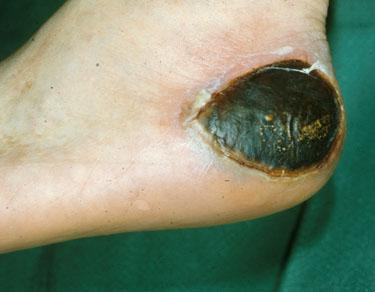
\includegraphics[keepaspectratio, width=3cm]{gambar/Bab3Extra/LukaHitam.jpg}
		\caption{Luka Hitam}
	\end{subfigure}
	\begin{subfigure}{.3\textwidth}
		\centering
		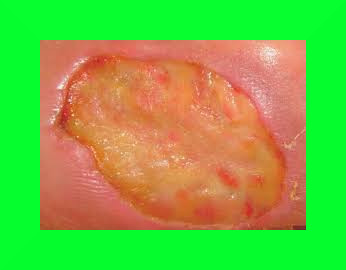
\includegraphics[keepaspectratio, width=3cm]{gambar/Bab3Extra/LukaKuning.jpg}
		\caption{Luka Kuning}
	\end{subfigure} 
	\begin{subfigure}{.3\textwidth}
		\centering
		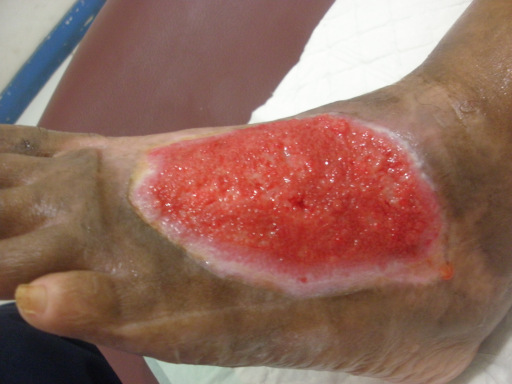
\includegraphics[keepaspectratio, width=3cm]{gambar/Bab3Extra/LukaMerah.jpg}
		\caption{Luka Merah}
	\end{subfigure}
	\caption{Data citra luka}
\end{figure}

\subsection{Validasi}

Seperti pada penelitian Rizki, akan diperiksa dahulu apakah hasil
pindai berhasil atau tidak. Setelah mendapatkan 
hasil deteksi keliling luka, harus divalidasi
ketepatan alat deteksi tersebut. penulis akan memvalidasi
data deteksi dengan menghitung selisih piksel dari hasil
alat deteksi, dengan \textit{ground truth} yang diambil dari
gambar manual menggunakan program GIMP.
similaritas akan dihitung sebagai berikut

\begin{equation}
  similiaritas(\%) = 100 - \left| \frac{luas \; ground \; truth - luas \; hasil \; deteksi}
  {luas \; ground \; truth} * 100  \right|
  \label{rumus:groundtruth}
\end{equation}

\begin{figure}[H]
	\centering
	\begin{subfigure}{.3\textwidth}
		\centering
		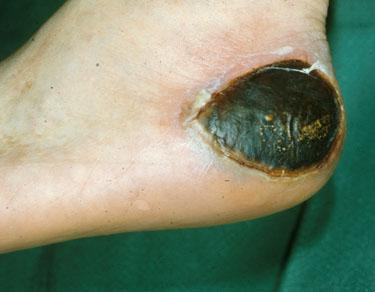
\includegraphics[keepaspectratio, width=3cm]{gambar/Bab3Extra/LukaHitam.jpg}
		\caption{Luka Hitam}
	\end{subfigure}
	\begin{subfigure}{.3\textwidth}
		\centering
		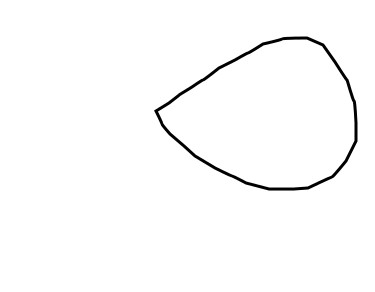
\includegraphics[keepaspectratio, width=3cm]{gambar/Bab3Extra/LukaHitamManual.jpg}
		\caption{Gambar Manual}
	\end{subfigure} 
	\begin{subfigure}{.3\textwidth}
		\centering
		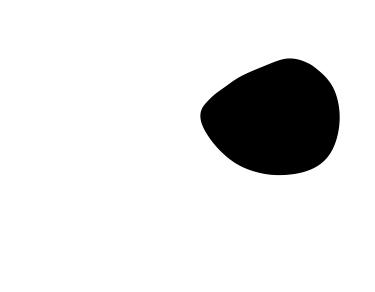
\includegraphics[keepaspectratio, width=3cm]{gambar/Bab3Extra/LukaHitamInt.jpg}
		\caption{Deteksi Interpolasi milik Rizki}
	\end{subfigure}
	\caption{Validasi alat deteksi}
\end{figure}

% Baris ini digunakan untuk membantu dalam melakukan sitasi
% Karena diapit dengan comment, maka baris ini akan diabaikan
% oleh compiler LaTeX.
\begin{comment}
  \bibliography{daftar-pustaka}
\end{comment}